\documentclass[11pt]{article}
\newcommand{\nombredocumento}{05 · Modelo realista}
% Preámbulo compartido por todos los documentos del proyecto (compilar con pdflatex).
\usepackage[utf8]{inputenc}
\usepackage[T1]{fontenc}
\usepackage{lmodern}
\usepackage{textcomp}
\usepackage[spanish,es-nodecimaldot,es-noshorthands,es-tabla]{babel}
\DeclareUnicodeCharacter{03A9}{\ensuremath{\Omega}}
\DeclareUnicodeCharacter{00B5}{\ensuremath{\mu}}
\DeclareUnicodeCharacter{03BC}{\ensuremath{\mu}}
\DeclareUnicodeCharacter{221A}{\ensuremath{\surd}}
\DeclareUnicodeCharacter{2192}{\ensuremath{\rightarrow}}
\DeclareUnicodeCharacter{2248}{\ensuremath{\approx}}
\DeclareUnicodeCharacter{2212}{\ensuremath{-}}
\DeclareUnicodeCharacter{2264}{\ensuremath{\le}}
\DeclareUnicodeCharacter{2265}{\ensuremath{\ge}}
\DeclareUnicodeCharacter{00D7}{\ensuremath{\times}}
\usepackage[a4paper,top=2.5cm,bottom=2.5cm,left=2.4cm,right=2.4cm,headheight=15pt]{geometry}
\setlength{\emergencystretch}{3em}
\usepackage{amsmath,amssymb,mathtools,bm}
\usepackage{siunitx}
\sisetup{output-decimal-marker={.},group-digits=false,per-mode=symbol,separate-uncertainty}
\usepackage{graphicx,float,booktabs,tabularx,longtable,array,multirow}
\usepackage[font=small,labelfont=bf]{caption}
\usepackage{enumitem}
\setlist{itemsep=2pt,topsep=4pt}
\usepackage[dvipsnames,table]{xcolor}
\usepackage[most]{tcolorbox}
\usepackage{tikz}
\usetikzlibrary{arrows.meta,positioning,shapes.geometric,calc,fit,backgrounds,decorations.markings}
\usepackage[european,straightvoltages]{circuitikz}
\usepackage{listings}
\usepackage{fancyhdr}
\usepackage{titlesec}
\usepackage{xurl}
\usepackage[colorlinks=true,linkcolor=Azul,urlcolor=Azul,citecolor=Azul]{hyperref}

\graphicspath{{../../simulacion/graficas/}{figuras/}}

% ---------------------------------------------------------------- colores
\definecolor{Azul}{HTML}{0D47A1}
\definecolor{Cian}{HTML}{00838F}
\definecolor{Naranja}{HTML}{E65100}
\definecolor{Rojo}{HTML}{C62828}
\definecolor{Verde}{HTML}{2E7D32}
\definecolor{Gris}{HTML}{455A64}
\definecolor{FondoCodigo}{HTML}{F5F7FA}

% ---------------------------------------------------------------- títulos
\titleformat{\section}{\Large\bfseries\color{Azul}}{\thesection}{0.8em}{}
\titleformat{\subsection}{\large\bfseries\color{Cian}}{\thesubsection}{0.8em}{}
\titleformat{\subsubsection}{\normalsize\bfseries\color{Gris}}{\thesubsubsection}{0.8em}{}

% ---------------------------------------------------------------- cabeceras
\pagestyle{fancy}
\fancyhf{}
\fancyhead[L]{\small\color{Gris}\nombredocumento}
\fancyhead[R]{\small\color{Gris}Generador de flujo axial con imanes NdFeB}
\fancyfoot[C]{\small\thepage}
\renewcommand{\headrulewidth}{0.4pt}

% ---------------------------------------------------------------- cajas
\newtcolorbox{nota}[1][Nota]{enhanced,breakable,colback=Azul!4,colframe=Azul!70,
  fonttitle=\bfseries,title={#1},left=6pt,right=6pt}
\newtcolorbox{advertencia}[1][Advertencia]{enhanced,breakable,colback=Rojo!4,colframe=Rojo!80,
  fonttitle=\bfseries,title={#1},left=6pt,right=6pt}
\newtcolorbox{resultado}[1][Resultado]{enhanced,breakable,colback=Verde!5,colframe=Verde!75,
  fonttitle=\bfseries,title={#1},left=6pt,right=6pt}
\newtcolorbox{paso}[1]{enhanced,breakable,colback=white,colframe=Cian!80,
  fonttitle=\bfseries,title={#1},left=6pt,right=6pt}

% ---------------------------------------------------------------- código
\lstdefinestyle{base}{
  basicstyle=\ttfamily\footnotesize,
  backgroundcolor=\color{FondoCodigo},
  frame=single,rulecolor=\color{Gris!40},
  breaklines=true,columns=fullflexible,keepspaces=true,
  keywordstyle=\color{Azul}\bfseries,
  commentstyle=\color{Verde}\itshape,
  stringstyle=\color{Naranja},
  showstringspaces=false,
  extendedchars=true,
  literate={á}{{\'a}}1 {é}{{\'e}}1 {í}{{\'i}}1 {ó}{{\'o}}1 {ú}{{\'u}}1 {ñ}{{\~n}}1
           {Á}{{\'A}}1 {É}{{\'E}}1 {Í}{{\'I}}1 {Ó}{{\'O}}1 {Ú}{{\'U}}1 {Ñ}{{\~N}}1
           {·}{{$\cdot$}}1 {→}{{$\rightarrow$}}1 {Ø}{{\O}}1 {Ω}{{$\Omega$}}1 {µ}{{$\mu$}}1
           {−}{{-}}1 {²}{{$^2$}}1 {√}{{$\surd$}}1 {≈}{{$\approx$}}1
}
\lstdefinestyle{python}{style=base,language=Python}
\lstdefinelanguage{JavaScript}{
  keywords={const,let,var,function,return,class,constructor,new,if,else,for,while,this,true,false,null,typeof,module,export,import},
  sensitive=true,comment=[l]{//},morecomment=[s]{/*}{*/},morestring=[b]',morestring=[b]",morestring=[b]`
}
\lstdefinestyle{js}{style=base,language=JavaScript}
\lstdefinestyle{consola}{style=base,keywordstyle=\color{black}}

% ---------------------------------------------------------------- utilidades
\newcommand{\vect}[1]{\mathbf{#1}}
\newcommand{\unitario}[1]{\mathbf{a}_{#1}}
\newcommand{\dif}{\mathrm{d}}
\DeclareUrlCommand\archivo{\urlstyle{tt}}
\makeatletter
\newcommand{\filasdesde}[1]{\@@input #1 }
\makeatother

\newcommand{\portada}[3]{%
  \begin{titlepage}
    \begin{tikzpicture}[remember picture,overlay]
      \fill[Azul] (current page.north west) rectangle ([yshift=-7cm]current page.north east);
      \node[anchor=north west,text=white,font=\sffamily\bfseries\Huge,text width=16cm,align=left]
        at ([xshift=2.4cm,yshift=-2.2cm]current page.north west) {#1};
      \node[anchor=north west,text=white!85!Azul,font=\sffamily\Large,text width=16cm,align=left]
        at ([xshift=2.4cm,yshift=-4.6cm]current page.north west) {#2};
    \end{tikzpicture}
    \vspace*{7cm}
    \begin{center}
      \begin{tikzpicture}[scale=0.9]
        \foreach \i in {0,...,7} {
          \pgfmathsetmacro{\ang}{45*\i}
          \ifodd\i \def\col{Azul!70}\def\pol{S}\else \def\col{Rojo!80}\def\pol{N}\fi
          \fill[\col] (\ang:2.2) circle (0.55);
          \node[white,font=\bfseries] at (\ang:2.2) {\pol};
        }
        \draw[Gris,line width=1pt] (0,0) circle (3.0);
        \fill[Gris!40] (0,0) circle (0.35);
      \end{tikzpicture}
    \end{center}
    \vfill
    {\large #3\par}
    \vspace{0.6cm}
    {\small\color{Gris}Basado en M.\,N.\,O. Sadiku, \emph{Elementos de Electromagnetismo}, 3.ª ed., Oxford University Press.\par
    Valores numéricos generados por el paquete \texttt{generador\_axial} (\texttt{uv run generador-axial reporte}).\par}
  \end{titlepage}
}

% Archivo generado automáticamente por `generador-axial reporte`. No editar a mano.
\newcommand{\ValGradoIman}{N38}  % Grado comercial del imán
\newcommand{\ValBr}{1.25}  % Remanencia [T]
\newcommand{\ValDiametroIman}{20}  % [mm]
\newcommand{\ValRadioIman}{10.0}  % [mm]
\newcommand{\ValEspesorIman}{5.0}  % [mm]
\newcommand{\ValAreaImanMM}{314.16}  % [mm^2]
\newcommand{\ValPolos}{8}
\newcommand{\ValParesPolos}{4}
\newcommand{\ValPasoPolarGrados}{45.0}  % [grados]
\newcommand{\ValRadioMontaje}{40.0}  % [mm]
\newcommand{\ValBobinas}{8}
\newcommand{\ValEspiras}{180}
\newcommand{\ValEspirasTotales}{1440}
\newcommand{\ValDiametroInteriorBobina}{12.0}  % [mm]
\newcommand{\ValDiametroExteriorBobina}{28.0}  % [mm]
\newcommand{\ValAlturaBobina}{6.0}  % [mm]
\newcommand{\ValEntrehierro}{2.5}  % [mm]
\newcommand{\ValEntrehierroMasAltura}{8.5}  % [mm]
\newcommand{\ValAcoplamiento}{0.85}
\newcommand{\ValCalibreAWG}{26}
\newcommand{\ValDiametroCobre}{0.404}  % [mm]
\newcommand{\ValDiametroEsmaltado}{0.455}  % [mm]
\newcommand{\ValAreaCobreMM}{0.1282}  % [mm^2]
\newcommand{\ValResistividadCobre}{1.72}  % [1e-8 ohm m]
\newcommand{\ValLongitudMediaEspira}{62.83}  % [mm]
\newcommand{\ValLongitudAlambreBobina}{11.31}  % [m]
\newcommand{\ValLongitudAlambreTotal}{90.48}  % [m]
\newcommand{\ValResistenciaBobina}{1.517}  % [ohm]
\newcommand{\ValResistenciaInterna}{12.14}  % [ohm]
\newcommand{\ValVentanaBobinaMM}{48.0}  % [mm^2]
\newcommand{\ValOcupacion}{0.78}
\newcommand{\ValRaizCaraIman}{11.1803}  % sqrt(L^2+R^2) [mm]
\newcommand{\ValTerminoCaraIman}{0.4472}  % L/sqrt(L^2+R^2)
\newcommand{\ValCampoCaraIman}{0.2795}  % [T]
\newcommand{\ValEntrehierroMasEspesor}{7.5}  % g+L [mm]
\newcommand{\ValRaizGL}{12.5000}  % sqrt((g+L)^2+R^2) [mm]
\newcommand{\ValRaizG}{10.3078}  % sqrt(g^2+R^2) [mm]
\newcommand{\ValTerminoUnoG}{0.6000}  % (g+L)/sqrt((g+L)^2+R^2)
\newcommand{\ValTerminoDosG}{0.2425}  % g/sqrt(g^2+R^2)
\newcommand{\ValCampoCaraBobina}{0.2234}  % [T]
\newcommand{\ValEntrehierroAlturaEspesor}{13.5}  % g+h+L [mm]
\newcommand{\ValRaizGHL}{16.8003}  % sqrt((g+h+L)^2+R^2) [mm]
\newcommand{\ValRaizGH}{13.1244}  % sqrt((g+h)^2+R^2) [mm]
\newcommand{\ValPrimitivaEnG}{2.1922}  % F(g) [mm]
\newcommand{\ValPrimitivaEnGH}{3.6759}  % F(g+h) [mm]
\newcommand{\ValDiferenciaPrimitivas}{1.4837}  % F(g+h)-F(g) [mm]
\newcommand{\ValCampoMedioBobina}{0.1545}  % [T]
\newcommand{\ValReduccionPorPromedio}{30.8}  % [%]
\newcommand{\ValFlujoMaximoMicro}{41.270}  % [uWb]
\newcommand{\ValAreaImanM}{3.1416}  % [1e-4 m^2]
\newcommand{\ValCaidaDiodo}{0.30}  % [V]
\newcommand{\ValCaidaPuente}{0.60}  % [V]
\newcommand{\ValCapacitanciaMicro}{220}  % [uF]
\newcommand{\ValTensionNominalCondensador}{50}  % [V]
\newcommand{\ValRpmMaxima}{1200}
\newcommand{\ValTensionDcMaxima}{29.27}  % [V]
\newcommand{\ValMargenCondensador}{41}  % [%]
\newcommand{\ValResistenciaLed}{2200}  % [ohm]
\newcommand{\ValPotenciaNominalResistenciaLed}{0.50}  % [W]
\newcommand{\ValCaidaLed}{2.0}  % [V]
\newcommand{\ValCorrienteLedRefMili}{2.21}  % [mA]
\newcommand{\ValCorrienteLedMaxMili}{12.4}  % [mA]
\newcommand{\ValCorrienteLedLimiteMili}{20}  % [mA]
\newcommand{\ValPotenciaResistenciaLedMax}{0.338}  % [W]
\newcommand{\ValRizadoRef}{251.4}  % [mV]
\newcommand{\ValRpmReferencia}{300}
\newcommand{\ValOmegaMecanicaRef}{31.416}  % [rad/s]
\newcommand{\ValFrecuenciaRef}{20.00}  % [Hz]
\newcommand{\ValPeriodoRefMs}{50.00}  % [ms]
\newcommand{\ValOmegaElectricaRef}{125.66}  % [rad/s]
\newcommand{\ValTensionPicoRef}{7.47}  % [V]
\newcommand{\ValTensionRmsRef}{5.28}  % [V]
\newcommand{\ValTensionDcRef}{6.87}  % [V]
\newcommand{\ValTensionPicoPorBobinaRef}{0.933}  % [V]
\newcommand{\ValRpmCarga}{400}
\newcommand{\ValOmegaMecanicaCarga}{41.89}  % [rad/s]
\newcommand{\ValTensionPicoCarga}{9.96}  % [V]
\newcommand{\ValTensionRmsCarga}{7.04}  % [V]
\newcommand{\ValCorrienteCarga}{0.290}  % [A]
\newcommand{\ValTensionEnCarga}{3.52}  % [V]
\newcommand{\ValPotenciaCarga}{1.021}  % [W]
\newcommand{\ValPotenciaPerdidas}{1.021}  % [W]
\newcommand{\ValPotenciaMecanica}{2.042}  % [W]
\newcommand{\ValParResistenteMili}{48.7}  % [mN m]
\newcommand{\ValEficiencia}{50}  % [%]
\newcommand{\ValBateriaTension}{12}  % [V]
\newcommand{\ValBateriaCapacidad}{7}  % [Ah]
\newcommand{\ValBateriaEnergia}{84}  % [Wh]
\newcommand{\ValBateriaResistencia}{0.05}  % [ohm]
\newcommand{\ValBateriaVacia}{11.8}  % E_oc con SoC = 0 [V]
\newcommand{\ValBateriaLlena}{12.8}  % E_oc con SoC = 1 [V]
\newcommand{\ValBateriaPendiente}{1.0}  % [V]
\newcommand{\ValSocInicial}{50}  % [%]
\newcommand{\ValSocCorte}{20}  % [%]
\newcommand{\ValSocReconexion}{25}  % [%]
\newcommand{\ValTensionOcRef}{12.30}  % [V]
\newcommand{\ValEnergiaUtilRef}{25.2}  % [Wh]
\newcommand{\ValControladorEficiencia}{90}  % [%]
\newcommand{\ValControladorArranque}{3.5}  % [V]
\newcommand{\ValControladorCorrienteMax}{3.0}  % [A]
\newcommand{\ValControladorAbsorcion}{14.4}  % [V]
\newcommand{\ValRpmMicrored}{600}
\newcommand{\ValFemRmsMicrored}{10.56}  % [V]
\newcommand{\ValTensionDcMicrored}{14.34}  % [V]
\newcommand{\ValPotenciaExtraibleMicrored}{2.297}  % [W]
\newcommand{\ValPotenciaHaciaBateria}{2.067}  % [W]
\newcommand{\ValCorrienteCargaMicroredMili}{168}  % [mA]
\newcommand{\ValPotenciaMecanicaMicrored}{4.59}  % [W]
\newcommand{\ValParMicroredMili}{73.1}  % [mN m]
\newcommand{\ValHorasRecarga}{20.8}  % [h]
\newcommand{\ValInversorTension}{110}  % [V]
\newcommand{\ValInversorPico}{155.6}  % [V]
\newcommand{\ValInversorTensionAlta}{220}  % [V]
\newcommand{\ValInversorPicoAlto}{311.1}  % [V]
\newcommand{\ValInversorFrecuencia}{60}  % [Hz]
\newcommand{\ValInversorNominal}{150}  % [W]
\newcommand{\ValInversorEficiencia}{90}  % [%]
\newcommand{\ValRelacionEspiras}{13.0}  % V_pico,AC / V_bat
\newcommand{\ValPotenciaCargaAc}{15}  % [W]
\newcommand{\ValCorrienteAcMili}{136}  % [mA]
\newcommand{\ValPotenciaEntradaInversor}{16.67}  % [W]
\newcommand{\ValCorrienteInversorBateria}{1.36}  % [A]
\newcommand{\ValPotenciaNetaBateria}{-14.60}  % [W]
\newcommand{\ValAutonomiaHoras}{1.73}  % [h]
\newcommand{\ValAutonomiaParadoHoras}{1.51}  % [h]
\newcommand{\ValRpmEquilibrio}{1704}
\newcommand{\ValPotenciaCargaReducida}{5}  % [W]
\newcommand{\ValRpmEquilibrioReducida}{984}
\newcommand{\ValInerciaRotor}{2.415}  % [1e-4 kg m^2]
\newcommand{\ValInductanciaBobinaMili}{0.528}  % [mH]
\newcommand{\ValInductanciaTotalMili}{4.22}  % [mH]
\newcommand{\ValFlujoMaximoReal}{0.827}  % phi_max normalizado
\newcommand{\ValPicoDerivadaFlujo}{0.746}
\newcommand{\ValRmsDerivadaFlujo}{0.559}
\newcommand{\ValFactorCresta}{1.335}
\newcommand{\ValFactorMedia}{0.706}
\newcommand{\ValRelacionFemRealIdeal}{0.930}
\newcommand{\ValPuntosRadiales}{32}
\newcommand{\ValMuestrasPerfil}{256}
\newcommand{\ValPasoIntegracionMili}{5}  % [ms]
\newcommand{\ValParCoulombMili}{3.0}  % [mN m]
\newcommand{\ValCoefViscosoMicro}{15.0}  % [uN m s]
\newcommand{\ValCoefVentilacionNano}{15.0}  % [nN m s^2]
\newcommand{\ValParMaximoMotriz}{0.30}  % [N m]
\newcommand{\ValVelocidadVacioMotriz}{1500}  % [RPM]
\newcommand{\ValParImpulso}{0.08}  % [N m]
\newcommand{\ValDuracionImpulso}{0.5}  % [s]
\newcommand{\ValCapacidadTermica}{100}  % [J/K]
\newcommand{\ValConveccionNatural}{8}  % [W/m^2K]
\newcommand{\ValConveccionForzada}{0.15}  % [W/m^2K por rad/s]
\newcommand{\ValCoefCobre}{0.393}  % [%/K]
\newcommand{\ValCoefRemanencia}{-0.12}  % [%/K]
\newcommand{\ValTemperaturaMaximaPla}{55}  % [C]
\newcommand{\ValBateriaRCero}{25}  % [mohm]
\newcommand{\ValBateriaRPolarizacion}{30}  % [mohm]
\newcommand{\ValBateriaTau}{30}  % [s]
\newcommand{\ValBateriaPeukert}{1.12}
\newcommand{\ValBateriaEtaCoulomb}{95}  % [%]
\newcommand{\ValBateriaEtaLlena}{60}  % [%]
\newcommand{\ValBateriaSocGas}{85}  % [%]
\newcommand{\ValBateriaAutodescarga}{3}  % [%/mes]
\newcommand{\ValBateriaSocFlotacion}{99.5}  % [%]
\newcommand{\ValBateriaFactorGas}{1500}
\newcommand{\ValBateriaPendienteGas}{50}
\newcommand{\ValControladorFlotacion}{13.8}  % [V]
\newcommand{\ValConsumoControladorMili}{8}  % [mA]
\newcommand{\ValInversorVacio}{3.6}  % [W]
\newcommand{\ValInversorCoefCuadratico}{5.81}  % [1e-4 1/W]
\newcommand{\ValInversorCorte}{10.8}  % [V]
\newcommand{\ValInversorReconexion}{12.3}  % [V]
\newcommand{\ValParReferencia}{0.07}  % [N m]
\newcommand{\ValRpmRegimenRef}{483}
\newcommand{\ValPotenciaEjeRef}{2.40}  % [W]
\newcommand{\ValPotenciaElectromagneticaRef}{2.21}  % [W]
\newcommand{\ValPerdidasCobreRef}{0.986}  % [W]
\newcommand{\ValPerdidasRozamientoRef}{0.192}  % [W]
\newcommand{\ValPerdidasFoucaultMili}{1.65}  % [mW]
\newcommand{\ValPotenciaBateriaRef}{0.96}  % [W]
\newcommand{\ValEficienciaRef}{40}  % [%]
\newcommand{\ValTensionDcRefReal}{3.50}  % [V]
\newcommand{\ValCorrienteGeneradorRef}{0.281}  % [A]
\newcommand{\ValTemperaturaRegimenRef}{27.8}  % [C]
\newcommand{\ValRpmConCargaRef}{483}
\newcommand{\ValPotenciaEntradaInversorRef}{18.7}  % [W]
\newcommand{\ValCorrienteNetaConCarga}{-1.48}  % [A]
\newcommand{\ValRpmParMaximo}{1002}
\newcommand{\ValPotenciaBateriaParMaximo}{4.35}  % [W]
\newcommand{\ValRizadoBajo}{18.8}  % [V] con 220 uF
\newcommand{\ValRizadoAlto}{0.88}  % [V] con 4700 uF
\newcommand{\ValRpmPicoImpulso}{505}
\newcommand{\ValTiempoParadaImpulso}{2.7}  % [s]
\newcommand{\ValHorasHastaAbsorcion}{4.0}  % [h]
\newcommand{\ValHorasHastaFlotacion}{8.2}  % [h]
\newcommand{\ValCorrienteFlotacionMili}{21}  % [mA]



\begin{document}

\portada{Modelo realista}
        {Dinámica del rotor, forma de onda real, electrónica con sus límites, batería de plomo-ácido, inversor y temperatura}
        {Documento 5 de 5 · Simulación dinámica del sistema completo}

\tableofcontents
\newpage

%=====================================================================
\section{Del modelo ideal al modelo realista}
%=====================================================================
Los Documentos~1 y~2 describen el generador en \textbf{régimen permanente} con hipótesis de libro de texto:
la velocidad se impone, el flujo es senoidal ($\Phi=k\bar B_zA\cos\theta_e$), la fuente tiene solo resistencia,
la batería es una fuente ideal con resistencia y el inversor tiene eficiencia constante. Esas hipótesis son
excelentes para dimensionar, pero no describen lo que se observa al construir el prototipo:
\begin{itemize}
  \item el rotor \textbf{no gira a la velocidad que uno quiere}: gira a la que resulta del equilibrio entre el par
        que se aplica, el rozamiento y el \textbf{frenado de Lenz} de la corriente que entrega;
  \item la fem \textbf{no es senoidal}: su forma la decide el solape geométrico entre el imán circular y la bobina;
  \item la batería \textbf{no es una fuente ideal}: su tensión sube al cargar (polarización), el controlador cambia
        de etapa (MPPT, absorción, flotación) y la capacidad depende de la corriente (Peukert);
  \item el inversor \textbf{consume aunque no haya carga} y se desconecta por baja tensión;
  \item las bobinas \textbf{se calientan}: la resistencia del cobre sube y el imán pierde remanencia.
\end{itemize}

El modelo realista integra en el tiempo todas esas físicas acopladas. Está implementado en Python
(\archivo{dominio/realista.py}, \archivo{dominio/dinamica.py}, \archivo{aplicacion/simulacion_dinamica.py}) y,
operación por operación, en el visualizador (\archivo{visualizador_3d/js/modelo/dinamica.js}). La prueba
\archivo{tests/test_paridad_visualizador.py} compara ambas implementaciones paso a paso en cuatro guiones
(arranque, absorción, flotación y corte por baja tensión) con tolerancia relativa $10^{-9}$.

\begin{figure}[H]
\centering
\begin{tikzpicture}[
  caja/.style={draw=#1,fill=#1!8,rounded corners=3pt,minimum height=0.95cm,align=center,font=\footnotesize,
               text width=2.3cm},
  flecha/.style={-{Stealth[length=2.2mm]},thick,Gris}]
  \node[caja=Azul] (eje) {Fuente motriz\\$\tau(\omega)$};
  \node[caja=Azul,right=0.5cm of eje] (rotor) {Rotor\\$J\,\dot\omega$};
  \node[caja=Naranja,right=0.5cm of rotor] (fem) {Fem real\\$-N\omega_e\,\phi'(\theta_e)$};
  \node[caja=Naranja,right=0.5cm of fem] (bob) {Bobinas\\$R(T),\ L$};
  \node[caja=Cian,below=1.3cm of bob] (puente) {Puente y $C$\\rizado};
  \node[caja=Cian,left=0.5cm of puente] (mppt) {Controlador\\de carga MPPT};
  \node[caja=Verde,left=0.5cm of mppt] (bat) {Batería\\Thévenin + $V_p$};
  \node[caja=Verde,left=0.5cm of bat] (inv) {Inversor\\$P_0+P+kP^2$};
  \node[caja=Rojo,right=0.9cm of bob,yshift=-1.12cm] (term) {Nodo térmico\\$C_t\,\dot T$};
  \draw[flecha] (eje) -- (rotor);
  \draw[flecha] (rotor) -- (fem);
  \draw[flecha] (fem) -- (bob);
  \draw[flecha] (bob) -- (puente);
  \draw[flecha] (puente) -- (mppt);
  \draw[flecha] (mppt) -- (bat);
  \draw[flecha] (bat) -- (inv);
  \draw[flecha,Rojo] (mppt.north) -- ++(0,0.45) -| node[pos=0.25,above,font=\scriptsize]{par de Lenz $P_{em}/\omega$} (rotor.south);
  \draw[flecha,Rojo] (bob.east) -| node[pos=0.25,above,font=\scriptsize]{$P_{Cu}+P_F$} (term.north);
  \draw[flecha,Rojo] (term.south) |- node[pos=0.75,below,font=\scriptsize]{$R(T)$, $B_r(T)$} (puente.east);
\end{tikzpicture}
\caption{Acoplamientos del modelo realista. Las flechas rojas son las realimentaciones que el modelo ideal ignora.}
\end{figure}

%=====================================================================
\section{Forma de onda real de la fem}
%=====================================================================
El imán es un disco de radio $r_m=\ValRadioIman$ mm y cada espira de la bobina es una circunferencia de radio
$\rho$ entre $D_i/2$ y $D_e/2$. Si $\bar B_z$ es uniforme sobre la huella del imán y nulo fuera de ella, el
flujo que concatena una espira es $\bar B_z$ por el área de intersección de dos círculos (una ``lente''):
\begin{multline*}
  A_{lente}(\rho,r_m,d)=\rho^2\arccos\frac{d^2+\rho^2-r_m^2}{2d\rho}+r_m^2\arccos\frac{d^2+r_m^2-\rho^2}{2dr_m}\\
  -\tfrac12\sqrt{(-d+\rho+r_m)(d+\rho-r_m)(d-\rho+r_m)(d+\rho+r_m)},
\end{multline*}
donde $d$ es la distancia entre centros. Al girar el rotor, los imanes de polaridad alterna pasan sobre la
bobina; sumando su contribución con signo y promediando sobre las espiras (repartidas uniformemente en $\rho$):
\[
  \phi(\theta_e)=\frac{\Phi}{\bar B_zA_{im}}=\frac{1}{A_{im}}\Big\langle\sum_k(-1)^kA_{lente}\big(\rho,r_m,d_k(\theta_e)\big)\Big\rangle_\rho,
  \qquad e(t)=-N_{total}\,\bar B_zA_{im}\,\omega_e\,\frac{d\phi}{d\theta_e}.
\]
El perfil se evalúa con \ValPuntosRadiales\ radios y \ValMuestrasPerfil\ muestras por periodo eléctrico.

\begin{resultado}[Resultado · forma de onda]
\begin{itemize}
  \item Flujo máximo normalizado $\phi_{max}=\ValFlujoMaximoReal$: confirma el factor de acoplamiento
        $k=\ValAcoplamiento$ que se supuso en el Documento~2.
  \item Factor de cresta de la fem $=\ValFactorCresta$ (una senoide tiene $\sqrt2=1.414$): la onda es
        \textbf{más aplanada}, casi trapezoidal.
  \item $E_{RMS,real}/E_{RMS,ideal}=\sqrt2\,\mathrm{rms}(\phi')/k=\ValRelacionFemRealIdeal$: el modelo ideal
        sobreestima la fem eficaz en un $\approx$7\,\%.
\end{itemize}
\end{resultado}

\begin{figure}[H]
\centering
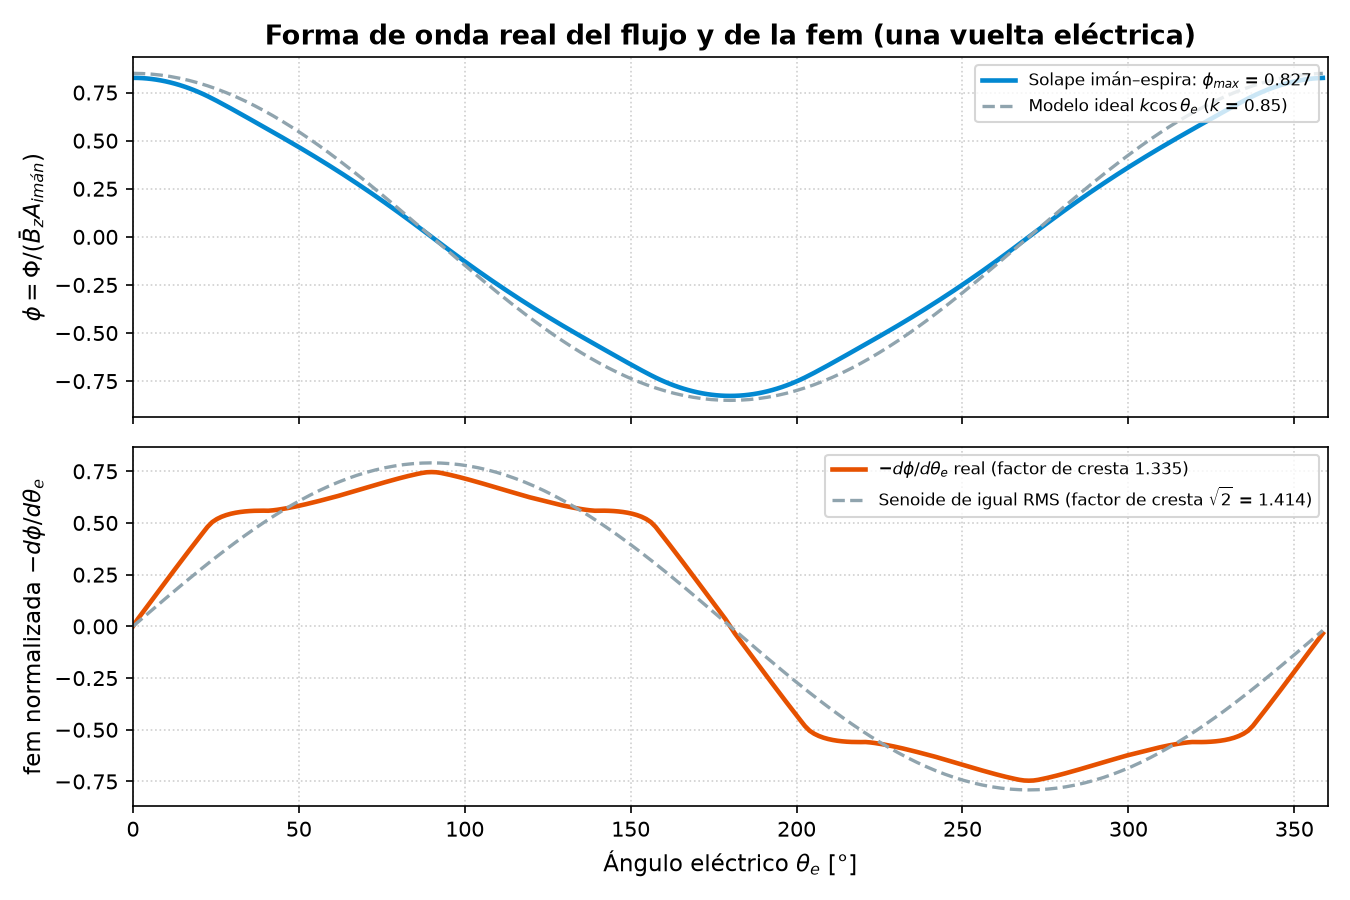
\includegraphics[width=0.85\linewidth]{09_onda_real_vs_senoidal.png}
\caption{Flujo normalizado y fem por solape imán–espira frente al modelo senoidal ideal.}
\end{figure}

%=====================================================================
\section{Circuito eléctrico con sus límites}
%=====================================================================
\subsection{Bobinas: resistencia con temperatura e inductancia}
\begin{gather*}
  R(T)=R_{20}\,\big[1+\alpha_{Cu}(T-20\,^\circ\text{C})\big],\qquad \alpha_{Cu}=\ValCoefCobre\ \text{\%/K};\\
  L_{bobina}=\frac{0.8\,N^2\bar r^2}{6\bar r+9h+10c}\ \text{(Wheeler, en pulgadas)}=\ValInductanciaBobinaMili\ \text{mH}.
\end{gather*}
Las ocho bobinas en serie suman $L=\ValInductanciaTotalMili$ mH, con reactancia $X=\omega_eL$. Como el estator
no tiene hierro, no hay par de retención (\emph{cogging}) ni histéresis; sí hay pequeñas corrientes de Foucault en
el propio cobre: $P_F=\ValPerdidasFoucaultMili$ mW a \ValRpmRegimenRef\ RPM.

\subsection{Puente rectificador, condensador y controlador MPPT}
Con corriente eficaz $I$, la potencia que llega al bus DC es
\[
  P_{DC}(I)=I\sqrt{E^2-X^2I^2}-RI^2-2V_D\,\bar I,\qquad \bar I=\tfrac{2\sqrt2}{\pi}I .
\]
El controlador busca $dP_{DC}/dI=0$ (bisección), pero no puede bajar el bus de \ValControladorArranque\ V, y
limita la potencia de salida por la tensión de la batería (absorción \ValControladorAbsorcion\ V; flotación
\ValControladorFlotacion\ V cuando SoC $\ge$ \ValBateriaSocFlotacion\,\%) y por corriente (\ValControladorCorrienteMax\ A).
El rizado del bus es
\[
  \Delta V=\frac{\bar I}{2f_eC}.
\]

\begin{advertencia}[Hallazgo · el condensador de 220 µF es insuficiente]
Con 0.2 N·m el rizado es de \ValRizadoBajo\ V con \ValCapacitanciaMicro\ µF y de \ValRizadoAlto\ V con 4700 µF.
El generador entrega corriente a baja frecuencia (decenas de Hz), por lo que el condensador debe ser de
miles de microfaradios. El visualizador lo señala con una alerta en la tarjeta de tensión DC y permite elegir
220, 1000, 2200 o 4700 µF.
\end{advertencia}

%=====================================================================
\section{Batería de plomo-ácido}
%=====================================================================
Se usa el circuito equivalente de Thévenin de primer orden (corriente $I>0$ cargando):
\begin{align*}
  V_{bornes}&=E_{oc}(\text{SoC})+V_p+R_0I, &
  \tau\,\dot V_p&=R_p(\text{SoC},I)\,I-V_p,\\
  R_p&=R_{p0}\,\big[1+A\,e^{B(\text{SoC}-1)}\big]\ (I>0), &
  \dot{\text{SoC}}&=\frac{\eta_c(\text{SoC})\,I}{C}\ \text{(carga)},\quad
  \dot{\text{SoC}}=-\frac{I_{ef}}{C}\ \text{(descarga)}.
\end{align*}

\begin{table}[H]
\centering
\caption{Parámetros de la batería (12 V, \ValBateriaCapacidad\ Ah, AGM).}
\begin{tabular}{llr}
\toprule
Símbolo & Descripción & Valor\\
\midrule
$R_0$ & Resistencia óhmica & \ValBateriaRCero\ m$\Omega$\\
$R_{p0}$, $\tau$ & Polarización (difusión del electrolito) & \ValBateriaRPolarizacion\ m$\Omega$, \ValBateriaTau\ s\\
$A$, $B$ & Sobrepotencial de gasificación al final de la carga & \ValBateriaFactorGas, \ValBateriaPendienteGas\\
$k_P$ & Exponente de Peukert (régimen C/20) & \ValBateriaPeukert\\
$\eta_c$ & Eficiencia coulómbica (por encima del \ValBateriaSocGas\,\% baja a \ValBateriaEtaLlena\,\%) & \ValBateriaEtaCoulomb\,\%\\
-- & Autodescarga & \ValBateriaAutodescarga\,\%/mes\\
\bottomrule
\end{tabular}
\end{table}

\begin{nota}[Acoplamiento implícito]
Al imponer la tensión de absorción, el controlador y la polarización de la batería forman un lazo muy rápido.
Con un paso explícito el lazo oscila; por eso la batería se evalúa con la polarización \emph{al final} del paso:
con retención $a=e^{-h/\tau}$, $E_{ef}=E_{oc}+V_pa$ y $R_{ef}=R_0+R_p(1-a)$. Es un esquema implícito exacto
para el circuito lineal, estable para cualquier factor de aceleración del tiempo.
\end{nota}

\begin{figure}[H]
\centering
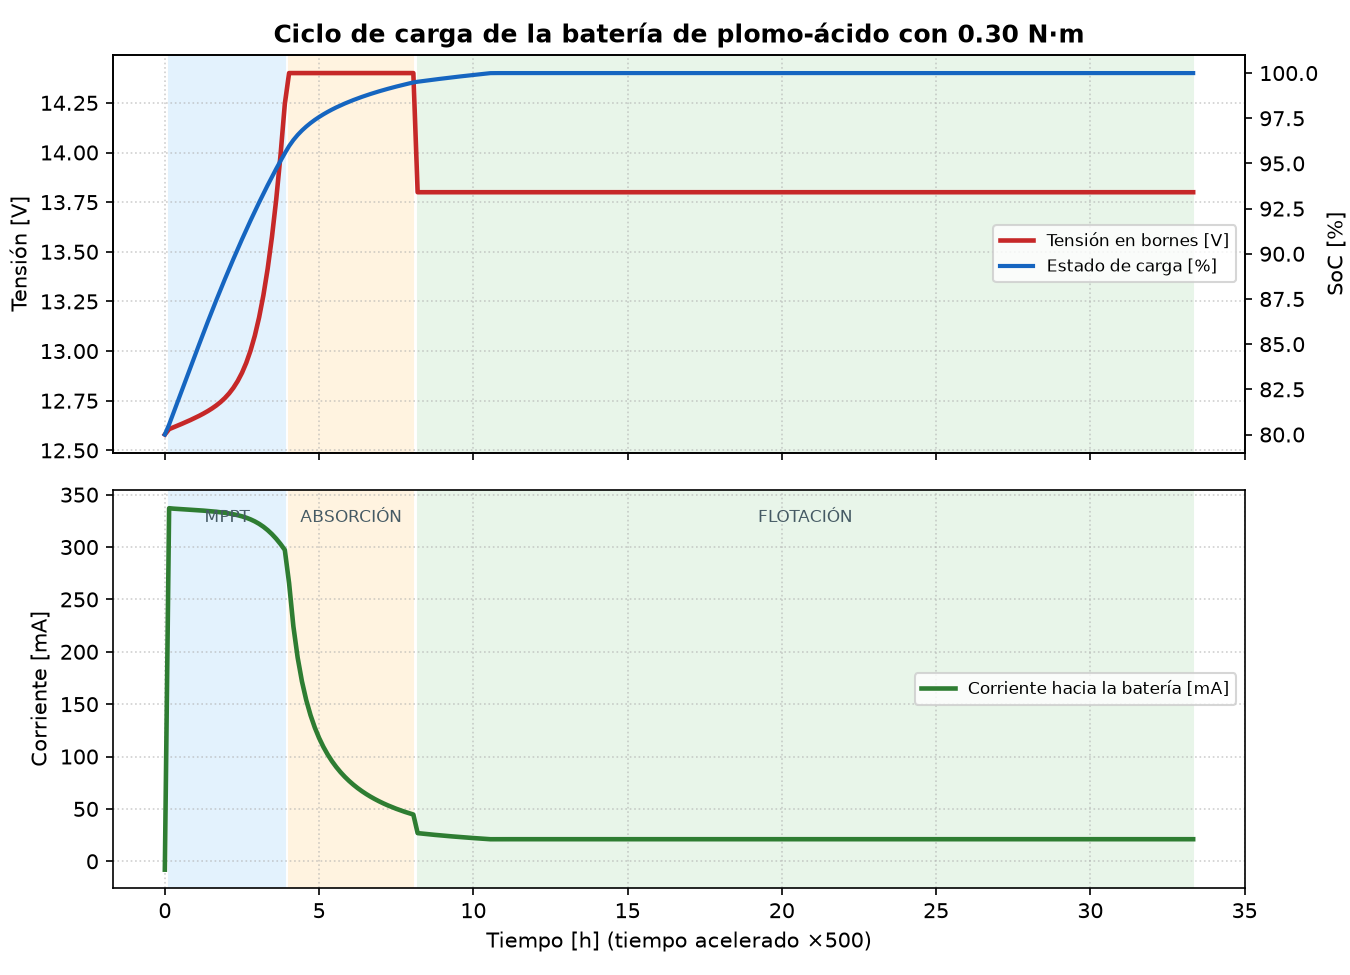
\includegraphics[width=0.85\linewidth]{12_ciclo_de_carga_bateria.png}
\caption{Ciclo de carga completo desde el 80\,\% con 0.30 N·m: MPPT hasta las \ValHorasHastaAbsorcion\ h, absorción
a \ValControladorAbsorcion\ V hasta las \ValHorasHastaFlotacion\ h y flotación con \ValCorrienteFlotacionMili\ mA.}
\end{figure}

%=====================================================================
\section{Inversor y controlador}
%=====================================================================
\[
  P_{entrada}=P_0+P_{AC}+k\,P_{AC}^2,\qquad P_0=\ValInversorVacio\ \text{W},\quad
  k=\ValInversorCoefCuadratico\times10^{-4}\ \text{W}^{-1}\ (\eta=\ValInversorEficiencia\text{\,\% a }\ValInversorNominal\ \text{W}).
\]
El inversor se desconecta cuando la tensión en bornes baja de \ValInversorCorte\ V y vuelve a conectarse por
encima de \ValInversorReconexion\ V (histéresis). El controlador consume \ValConsumoControladorMili\ mA de la
batería permanentemente. Con 15 W de carga el inversor toma \ValPotenciaEntradaInversorRef\ W: con
\ValParReferencia\ N·m la batería se descarga a \ValCorrienteNetaConCarga\ A.

%=====================================================================
\section{Dinámica del rotor}
%=====================================================================
\[
  J\,\dot\omega=\tau_{motriz}(\omega)-\frac{P_{em}+P_F}{\omega}-\tau_{roz}(\omega),\qquad
  \tau_{motriz}=\tau_{aj}\Big(1-\frac{\omega}{\omega_0}\Big),\qquad
  \tau_{roz}=T_c+b\,\omega+k_v\omega^2 .
\]
\begin{itemize}
  \item $J=\ValInerciaRotor\times10^{-4}$ kg·m² (disco de PLA menos los alojamientos, imanes NdFeB y eje de acero).
  \item Rozamiento de los rodamientos 608 y del aire: $T_c=\ValParCoulombMili$ mN·m (con rozamiento estático en
        reposo), $b=\ValCoefViscosoMicro$ µN·m·s, $k_v=\ValCoefVentilacionNano$ nN·m·s².
  \item Fuente motriz lineal (motor DC o manivela) con velocidad en vacío $\omega_0=\ValVelocidadVacioMotriz$ RPM
        y par ajustable hasta \ValParMaximoMotriz\ N·m.
  \item Integración con subpasos de \ValPasoIntegracionMili\ ms; las variables lentas (SoC, $V_p$, $T$) avanzan con
        el factor de aceleración del tiempo y la mecánica siempre en tiempo real.
\end{itemize}

\begin{resultado}[Resultado · régimen con \ValParReferencia\ N·m]
Velocidad \ValRpmRegimenRef\ RPM; potencia en el eje \ValPotenciaEjeRef\ W; potencia electromagnética
\ValPotenciaElectromagneticaRef\ W; pérdidas en el cobre \ValPerdidasCobreRef\ W y por rozamiento
\ValPerdidasRozamientoRef\ W; a la batería llegan \ValPotenciaBateriaRef\ W (eficiencia eje $\rightarrow$ batería
del \ValEficienciaRef\,\%). Con el par máximo (\ValParMaximoMotriz\ N·m) el rotor gira a \ValRpmParMaximo\ RPM y
carga con \ValPotenciaBateriaParMaximo\ W.
\end{resultado}

\begin{figure}[H]
\centering
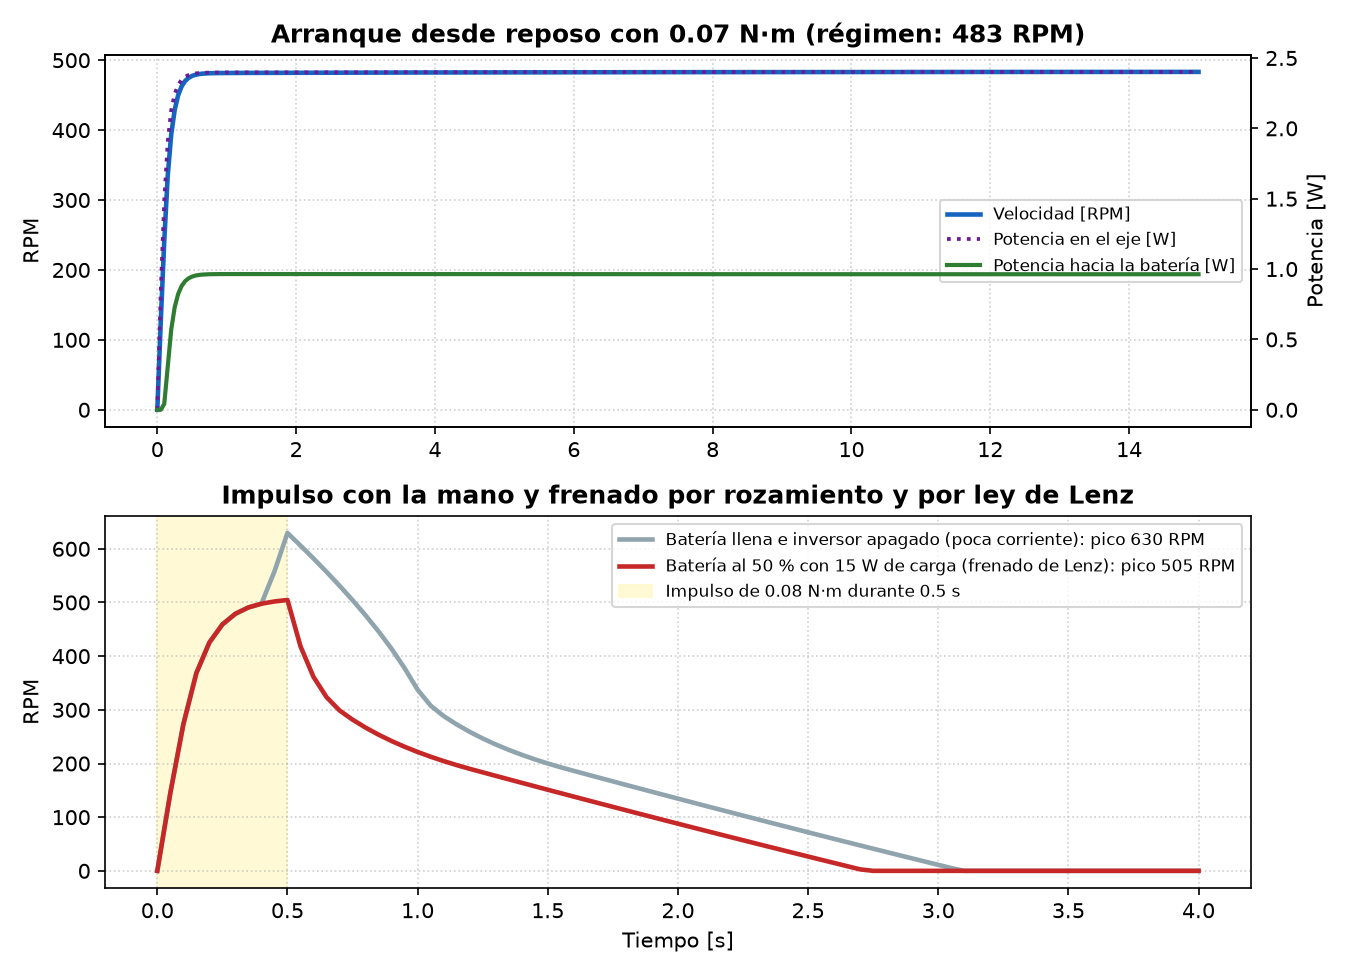
\includegraphics[width=0.85\linewidth]{10_arranque_impulso_y_frenado.png}
\caption{Arriba: arranque desde reposo. Abajo: impulso con la mano (\ValParImpulso\ N·m durante
\ValDuracionImpulso\ s): pico de \ValRpmPicoImpulso\ RPM y parada \ValTiempoParadaImpulso\ s después. La corriente
de carga frena el rotor (ley de Lenz).}
\end{figure}

\begin{figure}[H]
\centering
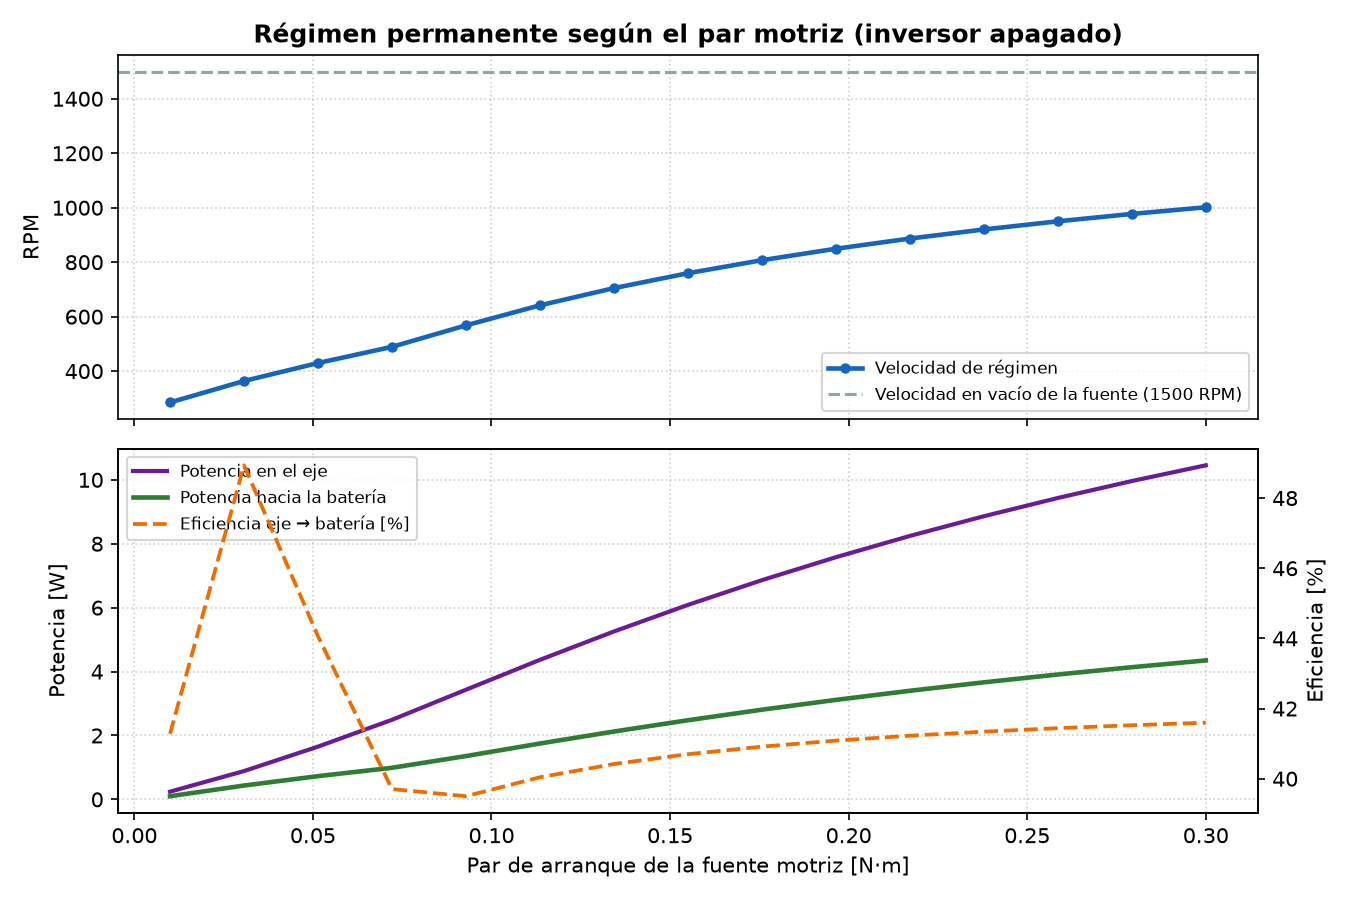
\includegraphics[width=0.85\linewidth]{11_regimen_vs_par_motriz.png}
\caption{Régimen permanente según el par. A bajo par el controlador queda limitado por la tensión mínima del bus
(\ValControladorArranque\ V) y opera con menos corriente, lo que explica el máximo local de eficiencia.}
\end{figure}

%=====================================================================
\section{Modelo térmico}
%=====================================================================
\[
  C_t\,\dot T=P_{Cu}+P_F-hA\,(T-T_{amb}),\qquad h=h_n+h_f\,\omega,\qquad
  B_r(T)=B_{r,20}\,\big[1+\alpha_B(T_{amb}-20\,^\circ\text{C})\big].
\]
Con $C_t=\ValCapacidadTermica$ J/K, $h_n=\ValConveccionNatural$ W/m²K, $h_f=\ValConveccionForzada$ W/m²K por
rad/s, $\alpha_B=\ValCoefRemanencia$\,\%/K. Con \ValParReferencia\ N·m las bobinas se estabilizan en
\ValTemperaturaRegimenRef\ °C; el visualizador avisa si superan \ValTemperaturaMaximaPla\ °C, temperatura a la que
el PLA empieza a ablandarse.

%=====================================================================
\section{Verificación}
%=====================================================================
\begin{itemize}
  \item \archivo{tests/test_modelo_realista.py}: geometría de la lente, perfil de flujo, Wheeler, inercia, MPPT,
        rizado, batería (polarización, Peukert, gasificación), inversor, validaciones, equilibrio de pares,
        \textbf{conservación de la energía} en cada paso, frenado de Lenz, etapas de carga, histéresis del corte y
        calentamiento.
  \item \archivo{tests/test_paridad_visualizador.py}: Python y JavaScript dan los mismos parámetros, perfil,
        inercia y serie temporal completa en cuatro guiones.
  \item \archivo{tests/test_interfaz_visualizador.py}: en un navegador real, cada control de la interfaz se acciona
        y lo que muestra el panel se compara con \texttt{SimulacionDinamica} de Python en el mismo estado.
\end{itemize}

\end{document}
